%!TeX root=../main.tex

\textbf{Continuous Control}\:
Weight agnostic neural networks (WANNs) are evaluated on three continuous control tasks.
%
The first, \texttt{CartPoleSwingUp}, is a classic control problem where, given a cart-pole system, a pole must be swung from a resting to upright position and then balanced, without the cart going beyond the bounds of the track.
%
The swingup task is more challenging than the simpler \texttt{CartPole}~\cite{openai_gym}, where the pole starts upright. Unlike the simpler task, it cannot be solved with a linear controller~\cite{tedrake2009underactuated,raiko2009variational}.
%
The reward at every timestep is based on the distance of the cart from track edge and the angle of the pole.
%
Our environment is closely based on the one described in \cite{gal2016improving,deepPILCOgithub}.

The second task, \texttt{BipedalWalker-v2}~\cite{openai_gym}, is to guide a two-legged agent across randomly generated terrain. 
%
Rewards are awarded for distance traveled, with a cost for motor torque to encourage efficient movement. 
%
Each leg is controlled by a hip and knee joint in reaction to 24 inputs, including LIDAR sensors which detect the terrain and proprioceptive information such as the agent's joint speeds. 
%
Compared to the low dimensional \texttt{CartPoleSwingUp}, \texttt{BipedalWalker-v2} has a non-trivial number of possible connections, requiring WANNs to be selective about the wiring of inputs to outputs.


The third, \texttt{CarRacing-v0}~\cite{openai_gym}, is a top-down car racing from pixels environment.
%
A car, controlled with three continuous commands (gas, steer, brake) is tasked with visiting as many tiles as possible of a randomly generated track within a time limit. 
%
Following the approach described in \cite{ha2018worldmodels}, we delegate the pixel interpretation element of the task to a pre-trained variational autoencoder~\cite{kingma2013auto,vae_dm} (VAE) which compresses the pixel representation to 16 latent dimensions. These dimensions are given as input to the network. 
%
The use of learned features tests the ability of WANNs to learn abstract associations rather than encoding explicit geometric relationships between inputs.
%, such as alternating hip movements of the \texttt{BipedalWalker-v2}. 

% -- %
% Experiment Methodology

%To uncover how well weight agnostic network architectures encode task solutions we compare their performance to hand designed network topologies applying various weight sampling and tuning techniques. We take the best performing weight agnostic network found over

Hand-designed networks found in the literature~\cite{ha2018designrl,ha2018worldmodels} are compared to the best weight agnostic networks found for each task. We compare the mean performance over 100 trials under 4 conditions:
\begin{enumerate}
\item \textit{Random weights}: individual weights drawn from $\mathcal{U}(-2,2)$;
%
\item \textit{Random shared weight}: a single shared weight drawn from $\mathcal{U}(-2,2)$; 
% 
\item \textit{Tuned shared weight}: the highest performing shared weight value in range $(-2,2)$;
%
\item \textit{Tuned weights}: individual weights tuned using population-based REINFORCE~\cite{williams1992simple}.
\end{enumerate}

%!TeX root=../main.tex

% Include # of connections? 
% Compress by taking 'Weight' out of table (Random|Random Shared|Tuned Shared|Tuned)

\begin{table}[h!]
\begin{small}
\vskip -0.05in % useful knobs to optimize layout
\caption      
{   
\textit{Performance of Randomly Sampled and Trained Weights for Continuous Control Tasks}
\newline
We compare the cumulative reward (average of 100 random trials) of the best weight agnostic network architectures found with standard feed forward network policies commonly used in previous work (i.e. \cite{ha2018designrl,ha2018worldmodels}). 
The intrinsic bias of a network topology can be observed by measuring its performance using a shared weight sampled from a uniform distribution.
By tuning this shared weight parameter we can measure its maximum performance.
To facilitate comparison to baseline architectures we also conduct experiments where networks are allowed unique weight parameters and tuned.
}
\label{table:rl_results}  
\begin{center}
\vskip -0.15in % useful knobs to optimize layout
\begin{tabular}{|c|c|c|c|c|}
\hline
{\textbf{Swing Up}} & \begin{tabular}[c]{@{}c@{}}Random Weights\end{tabular} & \begin{tabular}[c]{@{}c@{}}Random Shared Weight\end{tabular} & \begin{tabular}[c]{@{}c@{}}Tuned Shared Weight\end{tabular} & \begin{tabular}[c]{@{}c@{}}Tuned Weights\end{tabular} \\ \hline
WANN           & \textbf{57 $\pm$ 121} & \textbf{515 $\pm$ 58} & \textbf{723 $\pm$ 16}  & \textbf{ 932 $\pm$ 6} \\ \hline
Fixed Topology &         21 $\pm$ 43   & 7 $\pm$   2           &           8 $\pm$ 1    &          918 $\pm$ 7 \\ \hline
\end{tabular}

\vspace{1mm}

\begin{tabular}{|c|c|c|c|c|}
\hline
{\textbf{Biped}} & \begin{tabular}[c]{@{}c@{}}
Random Weights\end{tabular} & \begin{tabular}[c]{@{}c@{}}
Random Shared Weight\end{tabular} & \begin{tabular}[c]{@{}c@{}}
Tuned Shared Weight\end{tabular} & \begin{tabular}[c]{@{}c@{}}
Tuned Weights\end{tabular} \\ \hline
WANN           &   \textbf{-46 $\pm$ 54}   &    \textbf{51 $\pm$ 108 } & \textbf{261  $\pm$ 58}  & 332 $\pm$ 1  \\ \hline
Fixed Topology &  -129 $\pm$ 28            &  -107 $\pm$ 12            & -35  $\pm$ 23           & \textbf{347 $\pm$ 1}~\cite{ha2018designrl} \\ \hline
\end{tabular}

\vspace{1mm}

\begin{tabular}{|c|c|c|c|c|}
\hline
{\textbf{CarRacing}} & \begin{tabular}[c]{@{}c@{}}
Random Weights\end{tabular} & \begin{tabular}[c]{@{}c@{}}
Random Shared Weight\end{tabular} & \begin{tabular}[c]{@{}c@{}}
Tuned Shared Weight\end{tabular} & \begin{tabular}[c]{@{}c@{}}
Tuned Weights\end{tabular} \\ \hline
WANN           & \textbf{-69 $\pm$ 31}   & \textbf{375 $\pm$ 177}  & \textbf{608 $\pm$ 161}  & 893 $\pm$ 74  \\ \hline
Fixed Topology & -82 $\pm$ 13            & -85 $\pm$  27           & -37 $\pm$  36           & \textbf{906 $\pm$  21}~\cite{ha2018worldmodels} \\ \hline
\end{tabular}

\vspace{2mm}
\end{center}
\vskip -0.15in % useful knobs to optimize layout
\end{small}
\end{table}





% Expand on this paragraph?
The results are summarized in Table~\ref{table:rl_results}.\footnote{We conduct several independent search runs to measure variability of results in Supplementary Materials.}
%
In contrast to the conventional fixed topology networks used as baselines, which only produce useful behaviors after extensive tuning, WANNs perform even with random shared weights.
%
Though their architectures encode a strong bias toward solutions, WANNs are not completely independent of the weight values -- they do fail when individual weight values are assigned randomly.
%
WANNs function by encoding relationships between inputs and outputs, and so while the importance of the magnitude of the weights is not critical, their consistency, especially consistency of sign, is. An added benefit of a single shared weight is that it becomes trivial to tune this single parameter, without requiring the use of gradient-based methods.
% experiment with weights drawn from U[-2,0] or U[0,2]? 

The best performing shared weight value produces satisfactory if not optimal behaviors: a balanced pole after a few swings, effective if inefficient gaits, wild driving behaviour that cuts corners. 
%
These basic behaviors are encoded entirely within the architecture of the network. 
%
And while WANNs are able to perform without training, this predisposition does not prevent them from reaching similar state-of-the-art performance when the weights \textit{are} trained. 

%!TeX root=../main.tex


% TODO: 
% * To make clearer in gen 8 change 'step' to 'sig' and test again (it is illustrative anyway)
% * Color code neurons better


\begin{figure}[!htb]        
\vskip -0.00in % useful knobs to optimize layout
    \centering        
    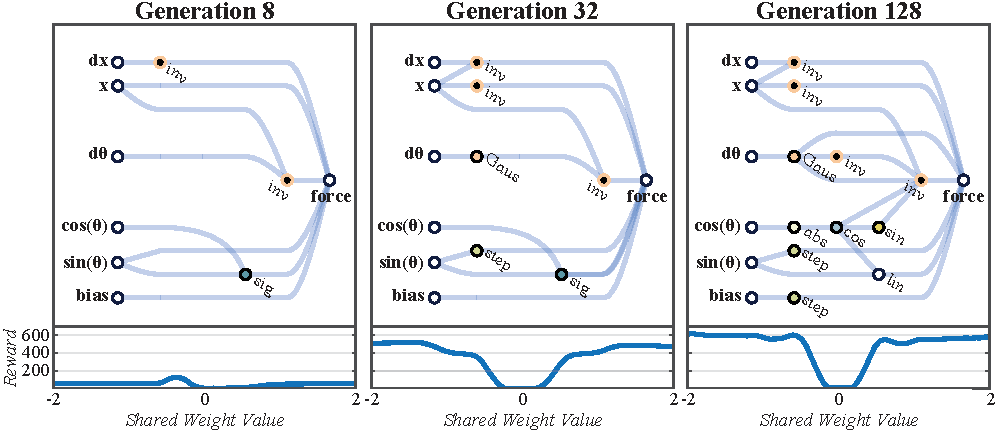
\includegraphics[width=1\textwidth]{img/swing.pdf}   
\vskip -0.05in % useful knobs to optimize layout
    \caption      
    {     
        \textit{Development of Weight Agnostic Neural Network Topologies Over Time}
        \newline
        \textit{Generation 8:} An early network which performs poorly with nearly all weights.
        \newline
        \textit{Generation 32:} Relationships between the position of the cart and velocity of the pole are established. The tension between these relationships produces both centering and swing-up behavior.
        \newline
        \textit{Generation 128:} Complexity is added to refine the balancing behavior of the elevated pole.
    }         
    \label{fig:swingNets}      
\vskip -0.05in % useful knobs to optimize layout
\end{figure}


As the networks discovered are small enough to interpret, we can derive insights into how they function by looking at network diagrams (See Figure~\ref{fig:swingNets}).
%
Examining the development of a WANN which solves \texttt{CartPoleSwingUp} is also illustrative of how relationships are encoded within an architecture. 
%
In the earliest generations the space of networks is explored in an essentially random fashion.
%
By generation 32, preliminary structures arise which allow for consistent performance: the three inverters applied to the $x$ position keep the cart from leaving the track. The center of the track is at $0$, left is negative, right is positive. 
%
By applying positive force when the cart is in a negative position and vice versa a strong attractor towards the center of the track is encoded.
%

% DH: may look at shortening this paragraph (or put it in the Appendix with extra figures)
The interaction between the regulation of position and the Gaussian activation on $d\theta$ is responsible for the swing-up behavior, also developed by generation 32. 
%
At the start of the trial the pole is stationary: the Gaussian activation of $d\theta$ is 1 and force is applied. 
%
As the pole moves toward the edge the nodes connected to the $x$ input, which keep the cart in the center, begin sending an opposing force signal.
%
The cart's progress toward the edge is slowed and the change in acceleration causes the pole to swing, increasing $d\theta$ and so decreasing the signal that is pushing the cart toward the edge.
%
This slow down causes further acceleration of the pole, setting in motion a feedback loop that results in the rapid dissipation of signal from $d\theta$.
%
The resulting snap back of the cart towards the center causes the pole to swing up.
%
As the pole falls and settles the same swing up behavior is repeated, and the controller is rewarded whenever the pole is upright.


As the search process continues, some of these controllers linger in the upright position longer than others, and by generation 128, the lingering duration is long enough for the pole to be kept balanced.
%
Though this more complicated balancing mechanism is less reliable under variable weights than the swing-up and centering behaviors, the more reliable behaviors ensure that the system recovers and tries again until a balanced state is found. % DH: this sentence is a bit hard to understand.
%
%Notably, as these behaviors are the result of tensions between systems set against each other, the particular magnitude of the weights makes little difference.
Notably, as these networks encode relationships and rely on tension between systems set against each other, their behavior is still consistent even with a wide range of shared weight values.
% DH: the above sentence is a bit hard to understand.
For video demonstrations of the policies learned at various developmental phases of the weight agnostic topologies, please refer to the \href{\websiteurl}{supplementary website}.

WANN controllers for \texttt{BipedalWalker-v2} and \texttt{CarRacing-v0} (Figure~\ref{fig:cover_diagram}, page 1) are likewise remarkable in their simplicity and modularity. 
%
The biped controller uses only 17 of the 25 possible inputs, ignoring many LIDAR sensors and knee speeds.
%
The WANN architecture not only solves the task without training the individual weights, but uses only 210 connections, an order of magnitude fewer than commonly used topologies (2804 connections used in the SOTA baseline~\cite{ha2018designrl}). 

The architecture which encodes stable driving behavior in the car racer is also striking in its simplicity (Figure~\ref{fig:cover_diagram}, right). 
%
Only a sparsely connected two layer network and a single weight value is required to encode competent driving behavior.
%
While the SOTA baseline \cite{ha2018worldmodels} also gave the hidden states of a pre-trained RNN world model, in addition to the VAE's representation to its controller, our controller operates on the VAE's latent space alone. Nonetheless, it was able to develop a feed-forward controller that achieves a comparable score. Future work will explore removing the feed-forward constraint from the search to allow WANNs to develop recurrent connections with memory states.

The networks shows in Figure~\ref{fig:cover_diagram}  (Page 1) were selected for both performance and readability. In many cases a great deal of complexity is added for only minimal gains in performance, in these cases we preferred to showcase more elegant networks. The final champion networks are shown in Figure~\ref{fig:nets}.

%!TeX root=../main.tex

\begin{figure}[ht!]
\vskip -0.00in % useful knobs to optimize layout
    \centering      
    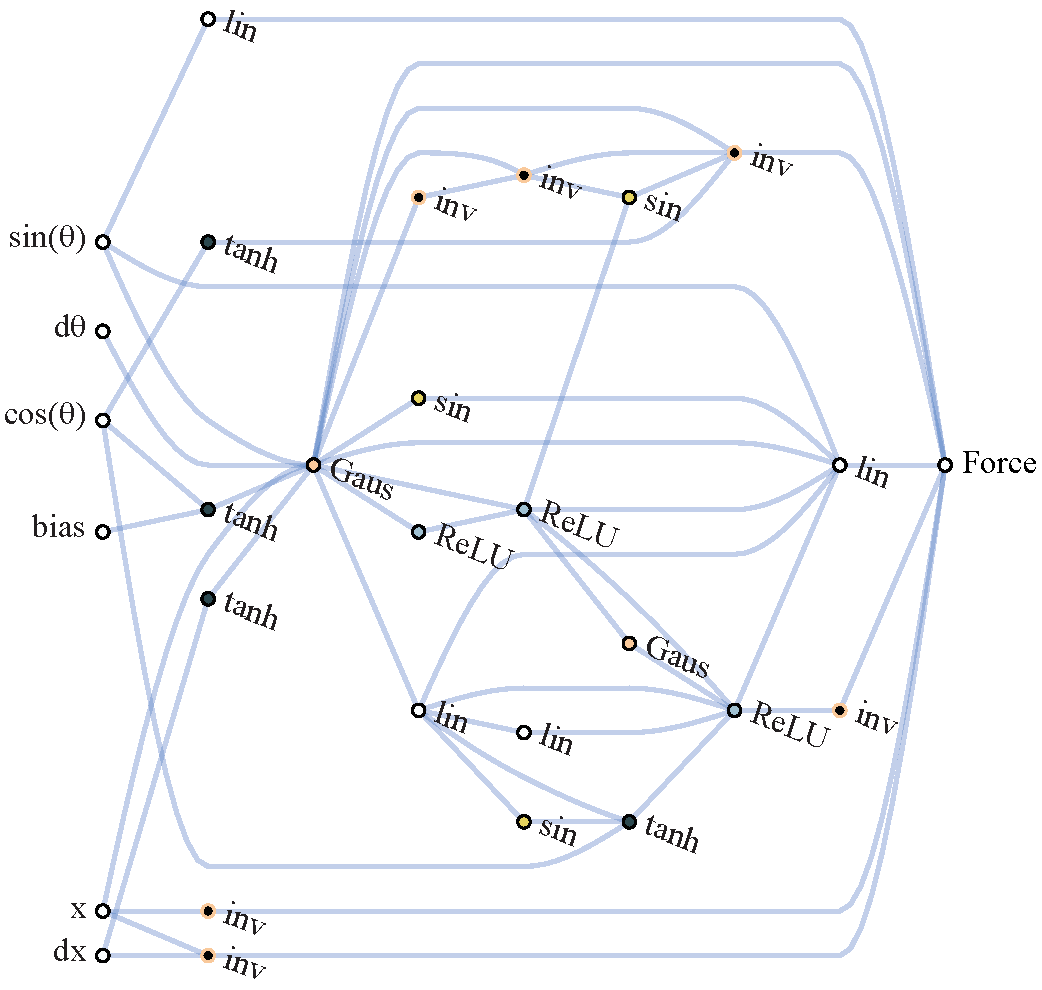
\includegraphics[width=0.32\textwidth]{img/champ_swingup.pdf}  
    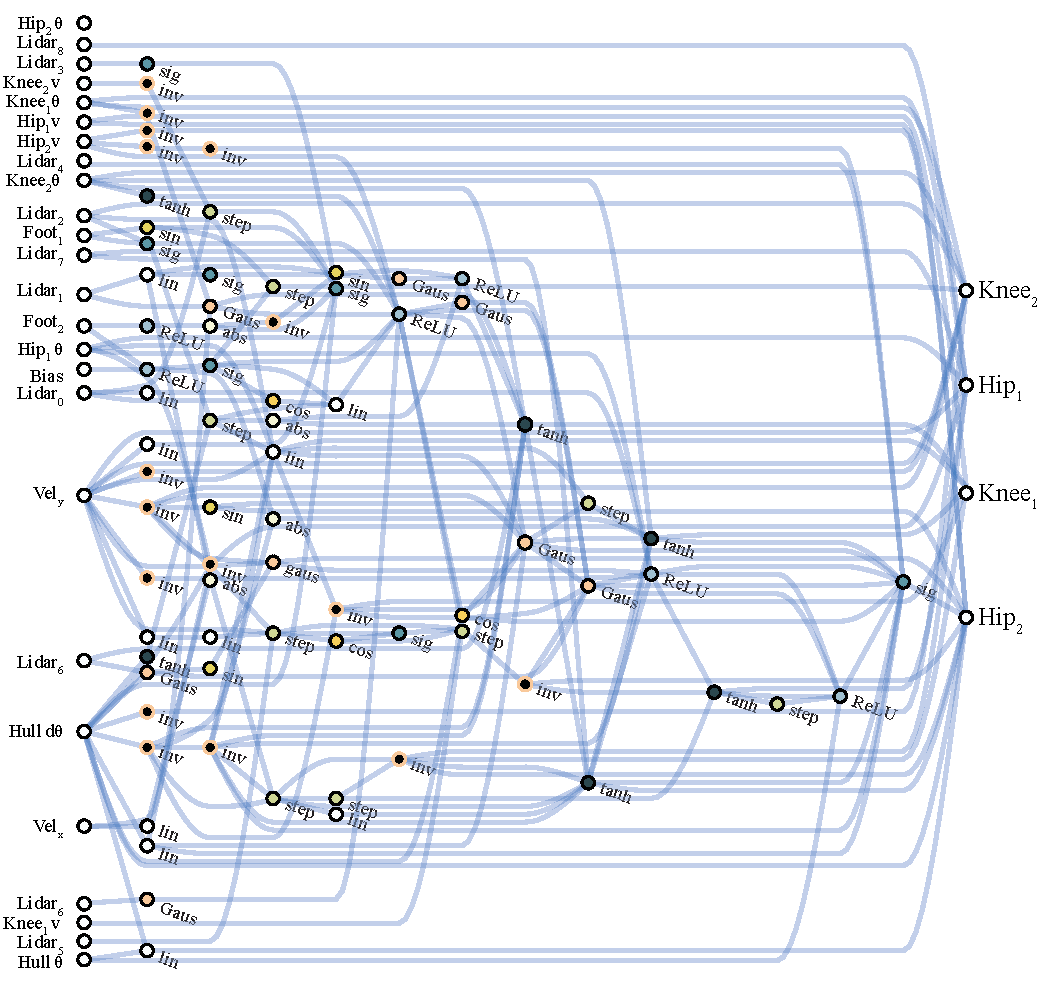
\includegraphics[width=0.32\textwidth]{img/champ_biped.pdf}  
    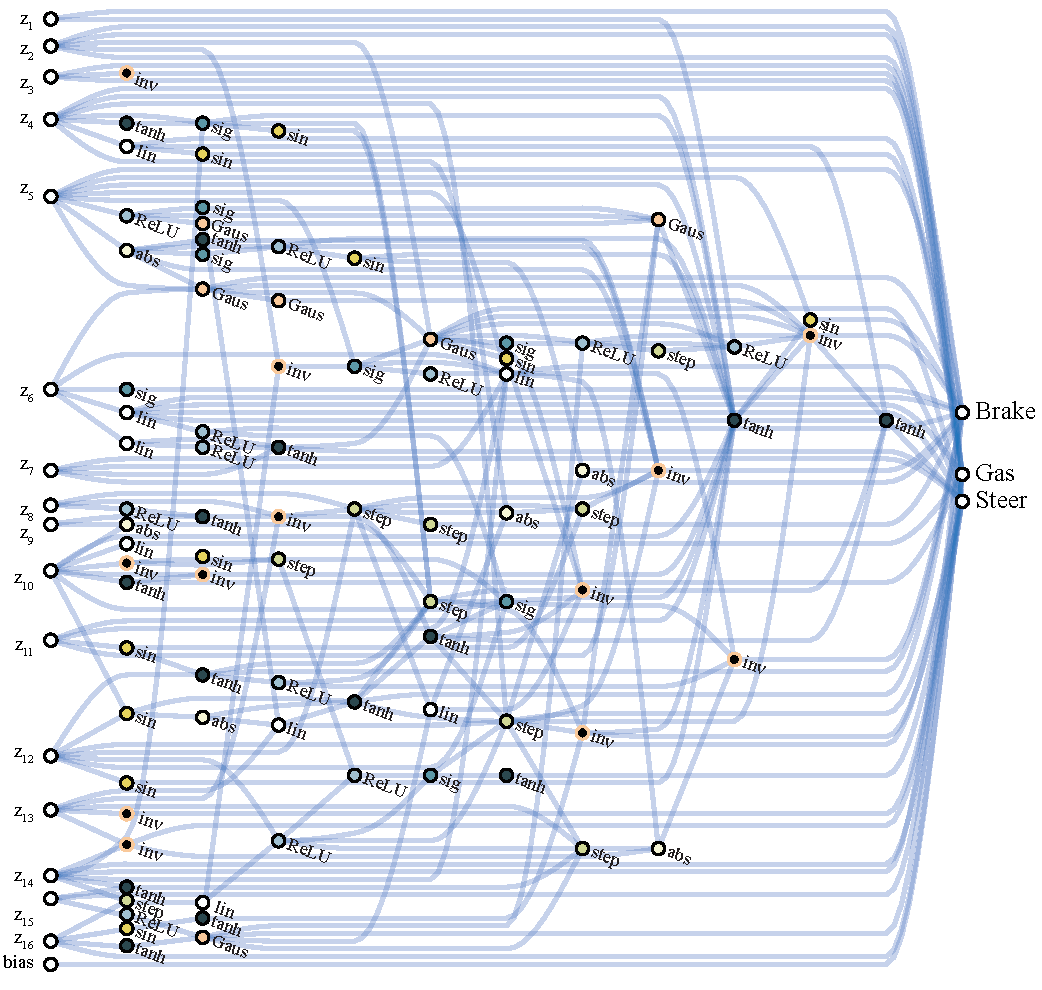
\includegraphics[width=0.32\textwidth]{img/champ_carracing.pdf}  
\vskip -0.00in % useful knobs to optimize layout
    \caption      
    {     
    \textit{Champion Networks for Continuous Control Tasks}
    \newline
	\textit{Left to Right (Number of Connections)}: Swing up (52), Biped (210), Car Racing (245)
    \newline
    Shown in Figure~\ref{fig:cover_diagram} (Page 1) are high performing, but simpler networks, chosen for clarity. The three network architectures in this figure describe the champion networks whose results are reported.
    }         
    \label{fig:nets}
\vskip -0.0in % useful knobs to optimize layout
\end{figure}

